\documentclass[12pt,a4paper]{article}
\usepackage[utf8]{inputenc}
\usepackage[spanish]{babel}
\usepackage{amsmath}
\usepackage{amsfonts}
\usepackage{amssymb}
\usepackage{graphicx}
\usepackage{kpfonts}
\usepackage[left=2cm,right=2cm,top=2cm,bottom=2cm]{geometry}
\title{EV 1-5 Características de los convertidores de potencia CA-CD, CD-CA, CA-CA y CD-CD}
\author{Giovanni Daniel Ruiz Tinoco\\
\small Sistemas electrónicos de interfaz\\
  \small Universidad Politécnica de la zona metropolitana de Guadalajara\\
  \small 4-B \\
  \small Ing. Mecatrónica\\
\centering

\includegraphics[scale=2]{imagenes/upz.jpg} 
}

\begin{document}
\maketitle
\newpage
\begin{center}
\section {Convertidor de potencia CA-CD}
\end{center}
Un convertidor de corriente alterna a corriente directa parte de un rectificador de onda completa.
El convertidor CA-CD nos proporciona una señal de salida rectificada (casi constante) de valor Vms donde Vm es igual al valor pico del voltaje de entrada.\\Este voltaje casi constante presenta una variación, que se puede considerar muy pequeño y de esta manera encontrar el valor del resistor del capacitor opara un valor de voltaje directo deseado.\\
\begin{center}
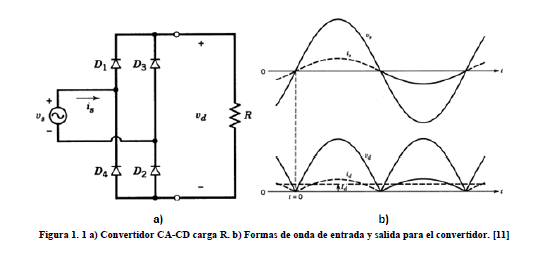
\includegraphics[scale=1]{imagenes/cacd.PNG} 
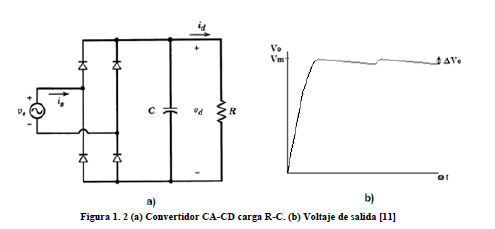
\includegraphics[scale=1]{imagenes/cacd2.PNG} 
\end{center}
\newpage
\begin{center}
\section {Convertidor de potencia CD-CA}
\end{center}
Los convertidores de corriente directa a corriente alterna son utilizados como drivers de motores como fuentes de corriente alterna ininterrumpida y tienen como objetivo producir una señal de corriente alterna sinusoidal, cuya magnitud y frecuencia puedan ser controladas. \\
Existen diversos tipos de convertidores inversores de los cuales el convertidor de una sola pierna y el convertidor en puente de media y onda completa, mostrados en las siguientes figuras son más comunes.\\
\begin{center}
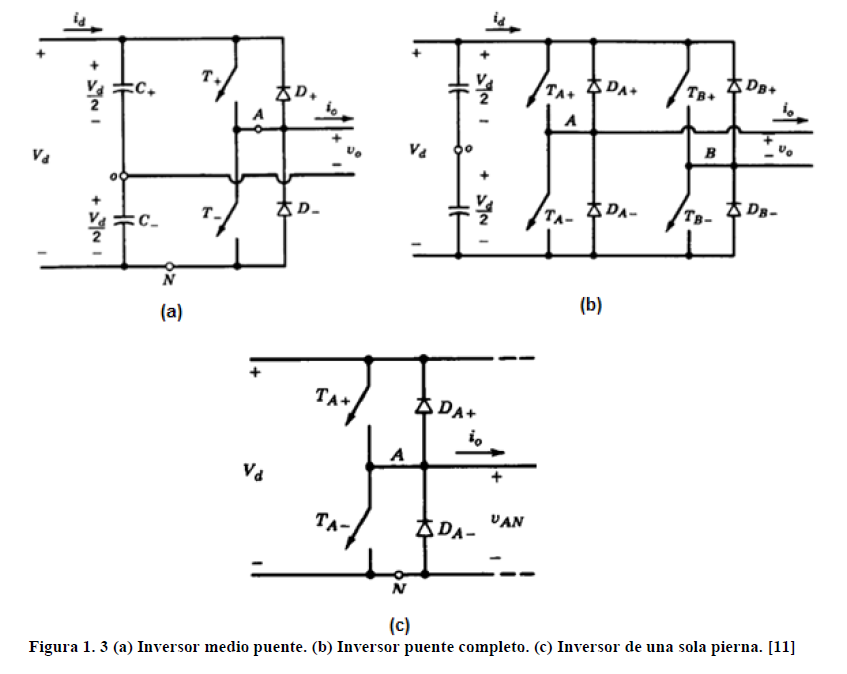
\includegraphics[scale=0.8]{imagenes/dcac1.PNG} 
\end{center}
\newpage
\begin{center}
\section{Convertidor de potencia CA-CA}
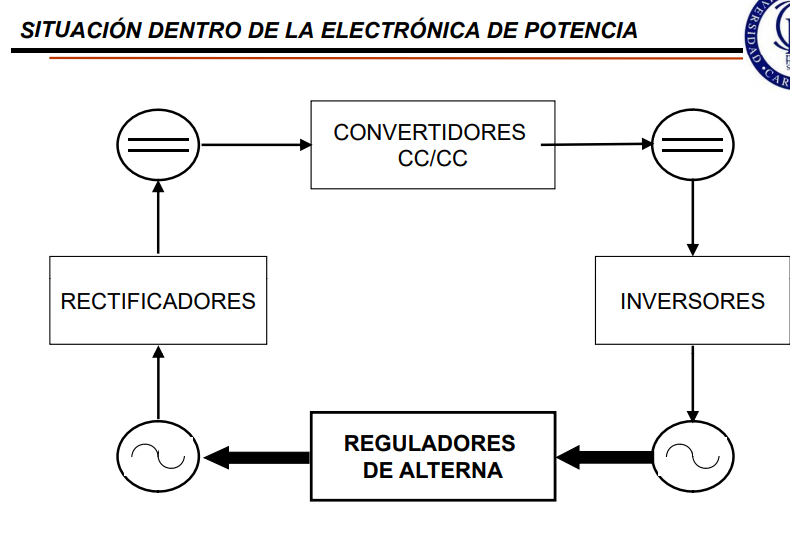
\includegraphics[scale=0.8]{imagenes/caca.PNG} 
\end{center}
\subsection{Caracteristicas de los reguladores de alterna\\}
\begin{flushleft}
-Realizan la conversión de AC/AC de forma directa y sin etapa intermedia de continua.\\
-Los tiristores no necesitan bloqueo reforzado gracias al paso natural por cero de la intensidad.\\ 
-Proporcionan una tensión de frecuencia fundamental menor o igual que la tensión de entrada.\\
-Proporcionan una tensión con un cierto contenido de armónicos.\\ 
\subsection{Clasificación de los reguladores de alterna}
\end{flushleft}
\begin{flushleft}
-Totales\\
-Diferenciales\\
-De fase\\
-Integral \\
-Cicloconvertidores\\
\end{flushleft}
\begin{center}
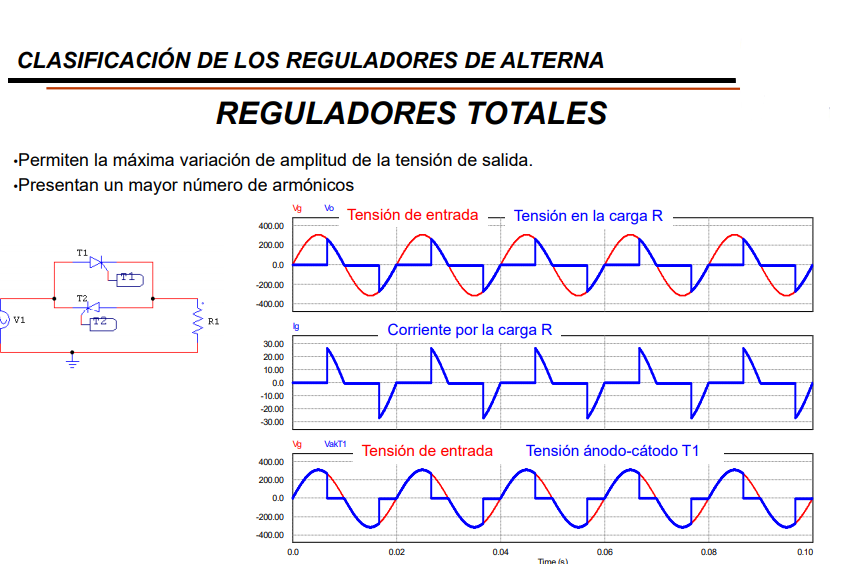
\includegraphics[scale=0.8]{imagenes/cacare.PNG}\\
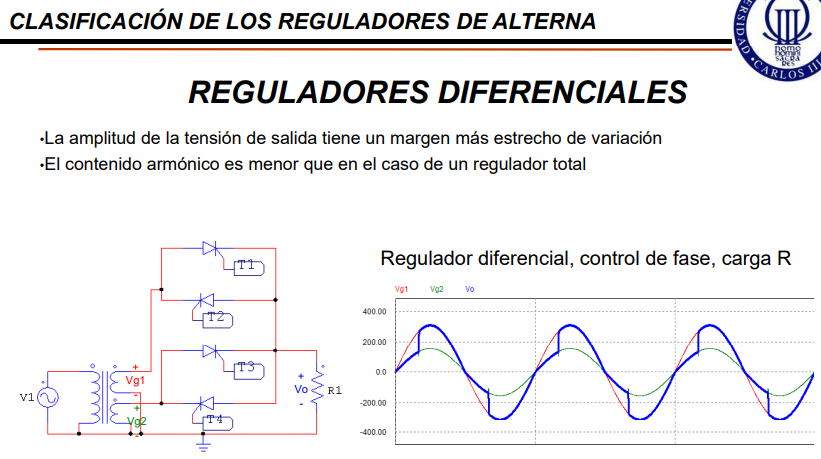
\includegraphics[scale=0.8]{imagenes/cacare2.PNG}\\ 
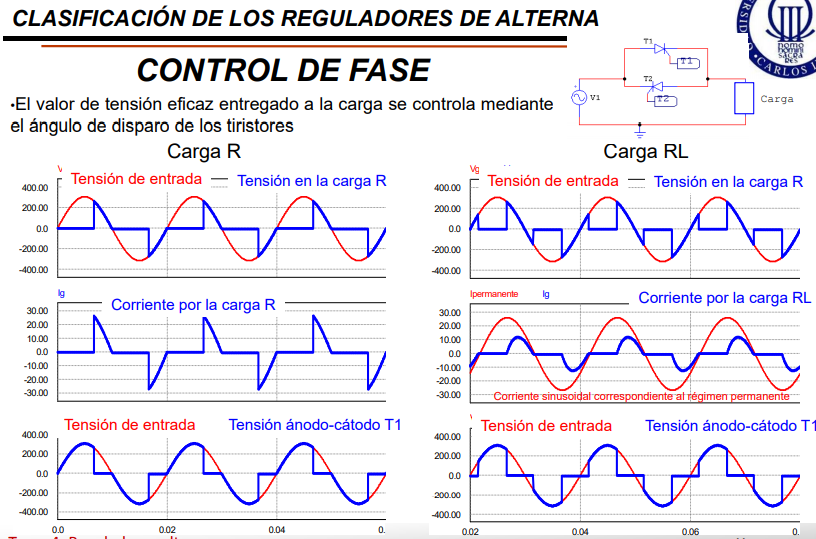
\includegraphics[scale=0.8]{imagenes/cacare3.PNG} 
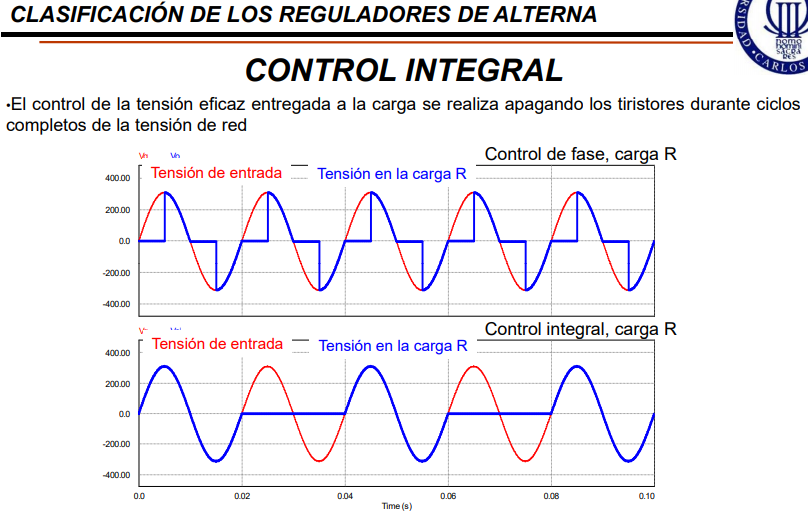
\includegraphics[scale=0.8]{imagenes/cacare4.PNG}
\end{center}
\newpage
\begin{center}
\section{Convertidores de potencia CD-CD}
\end{center}
\begin{flushleft}
Los convertidores CD-CD se utilizan ampliamente en el control de los motores de tracción de los automóviles eléctricos, tranvias eléctricos, grúas marinas, montacargas y elevadores de minas.\\
Un convertidor se puede utilizar para elevar un voltaje de CD. Cuando el interruptor de Q se cierra durante el tiempo T1, la corriente del inductor se eleva y la energía se almacena en el inductor L. Si durante el T2 el interruptor se abre, la energía almacenada de el inductor se transfiere a la carga a través del diodo D y la corriente del inductor se abate.
\begin{center}
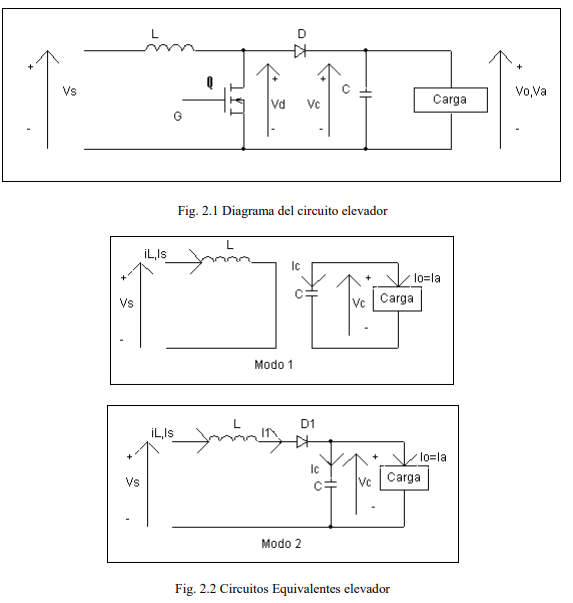
\includegraphics[scale=1]{imagenes/cdcdind.png} 
\end{center}
\newpage
La ecuación característica de este convertidor para determinar su voltaje de salida es: 
\begin{center}
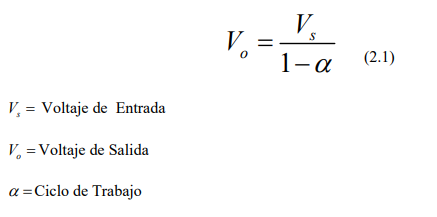
\includegraphics[scale=1]{imagenes/dcdc2.PNG} 
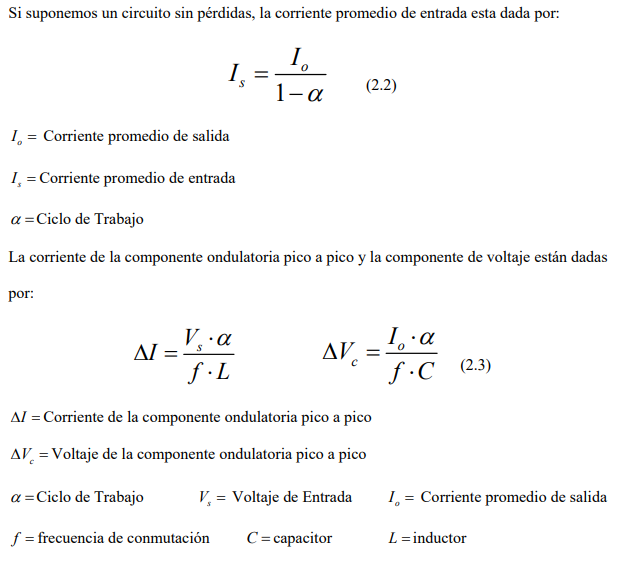
\includegraphics[scale=1]{imagenes/cdcd3.PNG} 
\end{center}
\end{flushleft}
Son varios los tipos de convertidores DC-DC existentes.\\ Normalmente se clasifican en tres grupos: los que disminuyen la tensión a su salida (convertidor reductor), los que aumentan la tensión a su salida (convertidor elevador) y los que son capaces de realizar ambas funciones.\\
\newpage
\end{document}

\section{se}